Active learning has emerged as a powerful paradigm in which labels of selected data points are sequentially queried from a large pool of unlabeled data, referred to as the unlabeled pool. The primary objective is to minimize labeling effort to find a classifier that exhibits low error on fresh data points from the same data source, known as generalization error. 
Typically, if the pool is large enough, a classifier that performs well on the pool can also achieve low generalization error through uniform convergence. 

Active learning has also been studied in the distributed setting, where the unlabeled pool is scattered across multiple machines (called agents), (e.g.,~\cite{shen2016distributed,aussel2020combining}). 
While active learning has demonstrated promising results, traditional approaches often operate in isolation, neglecting the potential benefits 
of collaboration among agents should they agree to collaborate. In this paper, we propose a novel framework for incentivized collaboration active learning, where agents can collaboratively explore their data pools to discover a common target function.
%

The motivation for collaboration in active learning stems from real-life scenarios where collaboration and collective intelligence yield improved outcomes, e.g., when agents collect data from the same distribution, and can easily end up labeling the same or very similar points. This redundancy leads to unnecessary and inefficient utilization of resources, as the labeling is often done by experts. Additionally, more data can be translated to improved accuracy, prompting agents to pool their resources and employ a more powerful model.

The incentive-driven nature of our framework aligns with the reality of collaboration in the real world. When agents are incentivized to collaborate only when their expected labeling complexity decreases, it reflects the real-life scenario where individuals are motivated to engage in cooperative endeavors if they perceive a clear benefit, such as reduced effort, faster, and better outcomes. In this work, we focus on a specific notion of incentives, where agents already have access to a baseline algorithm and they are motivated to join the collaboration if their label complexity is smaller than running the baseline algorithm on their own.

Consider, for example, the case of a new drug (e.g., Paxlovid for Covid-19~\citep{Paxlovid22}), that has different efficacy on patients with different features. While individual hospitals can test the drug on their patients in an active learning fashion by executing their preferred baseline algorithm, collaborating efficiently with other hospitals, each with their own patients, often leads to a better prognosis. 

However, if the incentives of the hospitals are not maintained, i.e., the effort of some hospitals is increased, the collaboration may be compromised. By emulating this collaboration within the active learning framework, we unlock the potential of collective intelligence to enhance the learning process. 
Besides, imagine that several data labeling companies have to recover the labels of unlabeled images assigned to them. Each data labeling company would like to collaborate with other companies to recover the labels of all images while minimizing the query complexity and not increasing their burden.
%






Our basic model is as follows: there are $k$ agents, each with their own set of unlabeled data points, and a single hypothesis class with a prior on the hypotheses, which all agents are aware of.
We assume realizability, meaning this hypothesis class encompasses a target function that accurately represents all the data points. 
The agents reach a consensus on an arbitrary baseline algorithm for pool-based active learning (e.g., the best tractable approximation algorithm).
To select whether or not to join the collaboration, the agents need to evaluate their utility from joining the collaboration. Since the goal of each individual agent (regardless of the collaboration) is to minimize their expected query complexity, the most natural cost function is the expected query complexity.
To ensure their individual benefits from their collaboration, we establish a collaboration protocol that guarantees that each agent cannot reduce their expected label complexity by running the baseline algorithm individually. This concept is referred to as individual rationality (IR). Our objective is to design an IR collaboration protocol that minimizes the overall labeling queries.




% [interesting examples]

There are cases in which collaboration is not necessarily beneficial. Suppose that no data point is shared by two agents (e.g., each agent has points on a different axis and the hypothesis class contains every possible halfspace). If the prior distribution is uniform over all labelings, then no agent can reduce their label complexity by joining the collaboration.

\begin{wrapfigure}[12]{R}{0.5\textwidth}
% \vspace{-2mm}
    \begin{minipage}{0.5\textwidth}
% \begin{figure}[t]
    \centering
    \scalebox{0.9}{
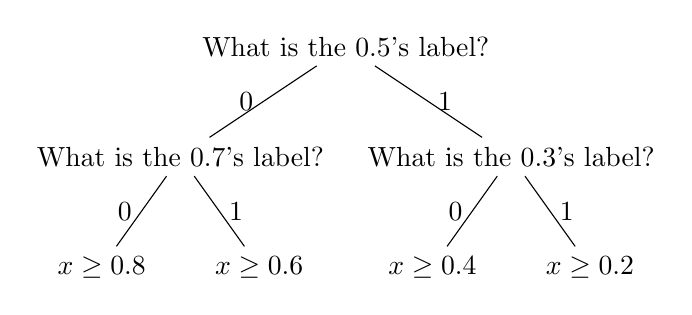
\begin{tikzpicture}[level distance=1.4cm,
  level 1/.style={sibling distance=4.2cm},
  level 2/.style={sibling distance=2cm}]

  \node (root) {What is the $0.5$'s label?}
    child {node (A) {What is the $0.7$'s label?}
      child {node (B) {$\ind{x\geq 0.8}$}}
      child {node (C) {$\ind{x\geq 0.6}$}}}
    child {node (D) {What is the $0.3$'s label?}
      child {node (E) {$\ind{x\geq 0.4}$}}
      child {node (F) {$\ind{x\geq 0.2}$}}};

  % Labels
  \path (root) -- (A) node[midway,left] {$0$};
  \path (root) -- (D) node[midway,right] {$1$};
  \path (A) -- (B) node[midway,left] {$0$};
  \path (A) -- (C) node[midway,right] {$1$};
  \path (D) -- (E) node[midway,left] {$0$};
  \path (D) -- (F) node[midway,right] {$1$};
\end{tikzpicture}}
    \caption{The query tree of binary search for thresholds.}
    \label{fig:query-tree}
% \end{figure}
\end{minipage}
\end{wrapfigure}
Clearly, if each agent has the same set of points, the label complexity of each agent can decrease to $1/k$ of its original label complexity if the collaboration protocol equally splits the labeling burden.
    Even if agents do not share the same set of points, they can still benefit from collaboration. For instance, consider the scenario with 1-dimensional thresholds $\cH =\{\ind{x\geq \alpha}|\alpha = 0.2,0.4,0.6,0.8\}$ and a uniform prior distribution over $\cH$. 
    Suppose agent 1 has points $\{0.25,0.5,0.75\}$ and agent 2 has points $\{0.3,0.45, 0.55, 0.7\}$. 
    When running binary search collaboratively, each agent only performs one labeling query, as illustrated as a search tree in Fig~\ref{fig:query-tree}. On the other hand, if they were to run binary search independently, each agent would need to query $2$ labels. Thus, collaboration can effectively reduce the label complexity for each agent by $1$.

 \textbf{Bayesian Assumption.} 
 The reason why we have a Bayesian assumption regarding the hypothesis class is that without it, querying all the labels to discover the target hypothesis can be inevitable, even for a simple class of linear separators in $\cR^2$ (see, e.g., Claim $1$ in~\citep{dasgupta2004analysis}).
It is worth noting that as in~\citep{dasgupta2004analysis}, we \textit{do not require the prior distribution to align with nature}. Instead, the prior distribution serves as a measure for average case analysis. Having a prior belief in our model has the following clear assumption. If the algorithm reaches a point where the remaining consistent hypotheses largely agree 
on the unlabeled data, it is reasonable to stop and output one of these remaining hypotheses~\citep{FreundSST97}. In a non-Bayesian setting, it does not make sense to operate this way. 

\textbf{Game Theory Interpretation.} 
%https://en.wikipedia.org/wiki/Mechanism_design
The agreed-upon baseline algorithm induces a sort of (not private) values for agents- each agent has its (negative) individual labeling complexity as value. 
The collaboration protocol can be then interpreted as a mechanism: 
Initially, the collaboration protocol (principal) is introduced to the agents, and each agent can understand it and have confidence in the principal's commitment to implementing it faithfully. Subsequently, the agents either rely on their trust in the algorithm's IR property or have the ability to verify it autonomously. Lastly, the agents behave in a rational manner by joining the collaboration only if it is IR.

We remark that there is an interesting parallelism between our IR collaboration algorithms and  truthful mechanisms. It is well known that Vickrey–Clarke–Groves (VCG) mechanism is a truthful mechanism that maximizes social welfare, but since it is hard to compute and to approximate~\citep{Buchfuhrer10}, the optimal outcome is replaced by a sub-optimal outcome of an approximation algorithm, and the resulting mechanism is not necessarily truthful. The goal is therefore relaxed to design an efficient approximation algorithm that returns a truthful mechanism. 





\textbf{Contributions and Organization.} We formalize the model in~\ref{sec:model}. In Section~\ref{sec:ir}, we demonstrate that any optimal algorithm is individually rational when the baseline is itself. This implies that optimizing for optimality ensures individual rationality for all baseline algorithms.

However, computing (or even approximating) the optimal algorithm is known to be NP-hard. To address this, we then show that the best available tractable approximation algorithm, the greedy algorithm \cite{kosaraju2002optimal,dasgupta2004analysis}, is not individually rational when the baseline is itself.
We demonstrate this by presenting an example where joining the collaboration increases the labeling complexity of an agent from $O(1)$ to $\Omega(n)$. 
In response, we introduce a general approach that can transform any arbitrary baseline algorithm into an IR collaborative algorithm. This conversion ensures that the total label complexity remains competitive with running the baseline algorithm on the entire data set. Furthermore, in Section~\ref{sec:sir} we present a scheme that converts any IR collaborative algorithm into a strict IR one, guaranteeing the label complexity is strictly lower by joining the collaboration under mild assumptions. 
When the baseline algorithm is both efficient and approximately optimal, our (strict) IR algorithms efficiently achieve label complexity that is approximately optimal.



